%  Robotics Text  by Jacob Rosen and Blake Hannaford
% (c) 2007  Jacob Rosen and Blake Hannaford
%

\chapter{Forward Kinematics}





\section{Problem Statement and Learning Objectives}
% Problem Statement and Learning Objectives for Chapter 03
\paragraph{Problem Statement}
 This chapter addresses the problem of computing the position and orientation of an end effector, knowing the geometry of the manipulator and the position values of each joint.  Joints may be rotary in which case the joint value is an angle, or prismatic, in which case the joint value is a displacement. We seek a general way to represent any serial manipulator. 

\paragraph{Learning Objectives}
 
After completing this chapter, the student will be able to derive the forward kinematic model of a serial manipulator.  Specifically to
\begin{itemize} 
  \item Identify the link and joint geometry from a picture or engineering drawing of a serial mechanism containing rotary and prismatic joints.
  \item Be able to assign a coordinate system to each link in a standardized manner. 
  \item Be able to derive Denavit-Hartenberg parameters for each link
  \item Be able to form the 4x4 homogeneous transform for each link based on the DH parameters and be able to multiply these link matrices together to get a symbolic expression for the forward kinematic equations in the form of a 4x4 homogenous transform matrix. 
\end{itemize}
The result is a computation of the position and orientation of the end effector knowing the geometric dimensions  of each link and the position of each joint in the mechanism.  






\section{Serial Mechanisms}

\subsection{Links and Joints}

\subsubsection{Links}
In this chapter we study the spatial relationships (transforms) between the links of a robot arm. First we define an {\it axis of motion} as
\begin{quotation}
A line in 3-space which contains points which are not moved by a particular rotation (a {\it rotary} axis), or which contains a direction describing linear motion (a {\it translation} axis).
\end{quotation}

We will define a {\it link} as
\begin{quotation}
A spatial relation, enforced by a rigid object, between two axes of motion.
\end{quotation}
In a typical robot arm, the links are rigid structural elements (most often of metal) which hold at each end the bearings for a joint.   Their rigidity enforces a constant spatial relationship between axes of motion at the {\it proximal} (closer to the base) and {\it distal} (closer to the end effector) ends.

\begin{figure}\centering
\includegraphics[width=2.75in]{figs03/00718.eps}
\caption{"Link", a rigid body which enforces a fixed spatial relationship between two axes of motion.}\label{LINK}
\end{figure}

\subsubsection{Joints}

Joints connect the links in a serial kinematic chain.  We define a joint as
\begin{quotation}
A structural element which allows relative motion between two bodies in only one degree of freedom.  Such motion is constrained to translational motion along a line or rotation around a line.
\end{quotation}

We have two classes of joints, {\it rotational} and {\it translational}, also known as {\it prismatic}\footnote
{Think of a prism sliding inside a hole shaped to match its profile.  It can slide in and out, but not rotate.}.   Combining the definitions of link and joint, we see that each axis of motion is fixed in the two links adjoining the joint.   The degree of translation or rotation (the single motion freedom of the joint) is called the joint variable.    Since the joint constrains relative motion of the two links to a single degree of freedom, the joint variable is sufficient to describe the spatial relationship between them.


\begin{figure}\centering
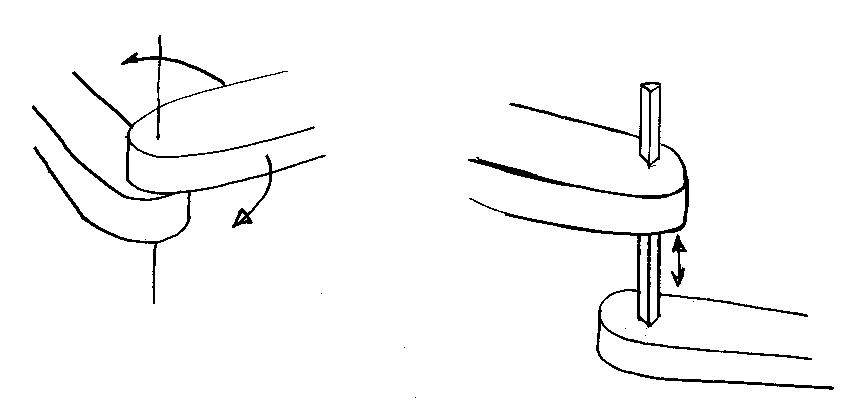
\includegraphics[width=3.5in]{figs03/00341.eps}
\caption{Two types of joints, rotational and translational/prismatic.}\label{RotationalTranslationalJoints}
\end{figure}


A series of such links bridging adjacent axes is an open kinematic chain (also known as a robot arm!).
The {\it forward kinematics} problem is to find the position and orientation of the last link in the chain (i.e. the robot hand) knowing only the robot's geometry and the angles or displacements of the joints. To make our method general, we will assume that there can be any amount of twist, displacement, and offset between the ends of each link. This make the problem difficult unless we employ a systematic approach.  We will use the approach invented by Denavit and Hartenberg in which we will construct a virtual kinematic chain which is equivalent to the original robot but is easier to analyze.  The virtual kinematic chain in the ``DH" method consists of the joint axes and their {\it common normals}.   The common normal between two lines or axes is a unique\footnote{Not always unique but see below.} line which is perpendicular to both axes.




\subsection{Modeling Links and Joints}


\begin{figure}
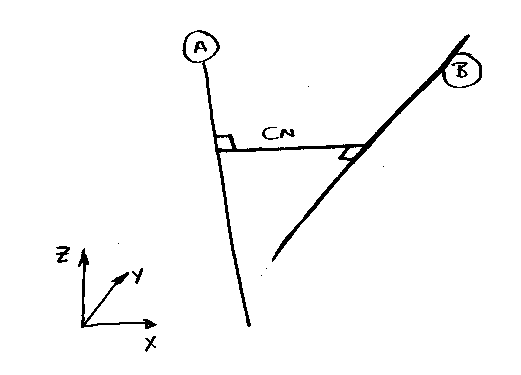
\includegraphics[width=3.5in]{figs03/00337.eps}
\caption{The Common Normal (CN) is the shortest line which intersects two given lines.  It intersects  lines {\bf A} and {\bf B}  at a right angle.}\label{CommonNormals}
\end{figure}


\begin{figure}
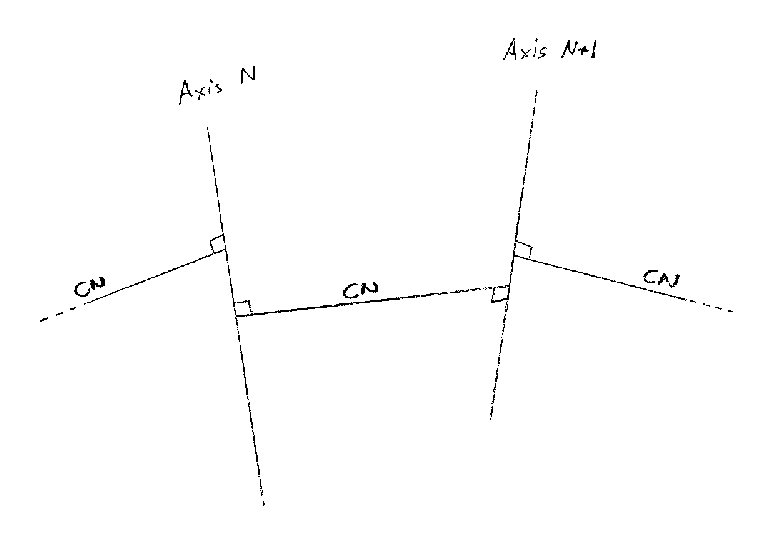
\includegraphics[width=3.5in]{figs03/00339.eps}
\caption{Virtual Links between axes are formed by the Common Normals.}\label{VirtualLinksCN}
\end{figure}

\subsubsection{Assignment of Frames to Links}
We will define a series of frames along the virtual kinematic chain and identify the key rotations and translations which define their relationships.


\paragraph{Common Normal}

The CN will be our virtual link between two axes in space.   It is worth noting that the CN might be completely outside the physical structure of the robot.  However our virtual manipulator constructed using CNs will be an exact representation of the kinematics of the real one.   It turns out that we can identify the CN of each link rather informally.  We do not need to write the equation for each CN line segment but it will be more important to identify the two end points.

There will be a CN for each pair of joint axes (Figure \ref{VirtualLinksCN}).  If the two joint axes are parallel, there are an infinite number of CNs so we just choose one arbitrarily.  If the two axes intersect, then the CN has zero length but it still has a direction which is the cross product

\begin{equation}
CN = \mathrm{Axis}_N \otimes \mathrm{Axis}_{N+1}
\end{equation}


%%%%%%%%%%%%%%%%%%%%%%%%%%%%%%%%%%%%%%%%%%%%%%%%%%%%%%%%%%%%%%%%%%%%%%%%%%%%%%%%%%%%%%%%%%%%%%%%%%%%%%%%%%
\begin{ExampleSmall}
Find the Common Normal between the following lines:
\[
x=0, y=0
\]
and
\[
z=1, x=1
\]

The common normal is also the shortest line segment which intersects both lines.   The first line is a vertical along the $z$ axis.  The second goes in the $y$ direction through the point $[1 \quad 0\quad 1]^T$.    The shortest line segment connecting these two lines is the line segement between $[0\quad 0\quad 1]^T$ and $[1\quad 0\quad 1]^T$ which is the line
\[
z=1, y=0
\]

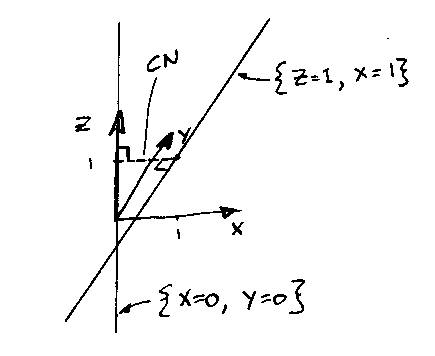
\includegraphics[width=2.5in]{figs03/00338.eps}

\end{ExampleSmall}



\subsection{Fixing Frames to Links}

Once we identify common normals between the manipulator axes, we are ready to locate a frame, rigidly attached to each link.  Although conceptually these could be anywhere, our convention will locate them on the joint axes.  We will  first choose the location of the origin, and then the directions for two axes.   The third axis follows by the right hand rule.


The origin of the link frame will be at the point where Axis $N$ intersects the CN to Axis $N+1$.  Let's call this point $A_N$.    The $X_N$ axis will point along the CN toward its intersection with the following axis.  Let's call the other end of the CN $B_N$.   $Z_N$ will point along the joint axis.  There are two ways that $Z_N$ can point along $Z_N$.    For rotary joints, we will require that we choose the direction of $Z_N$ so that positive rotation of the joint is consistent with the right-hand-rule about $Z_N$.  The points $A_N$ and $B_N$ are shown in Figure \ref{VirtualLinkswFrames}.

Now that $X_N$ and $Z_N$ are fixed, we choose $Y_N$ simply by
\[
Y_N = Z_N \otimes X_N
\]

\begin{figure}[p]
\centering
A)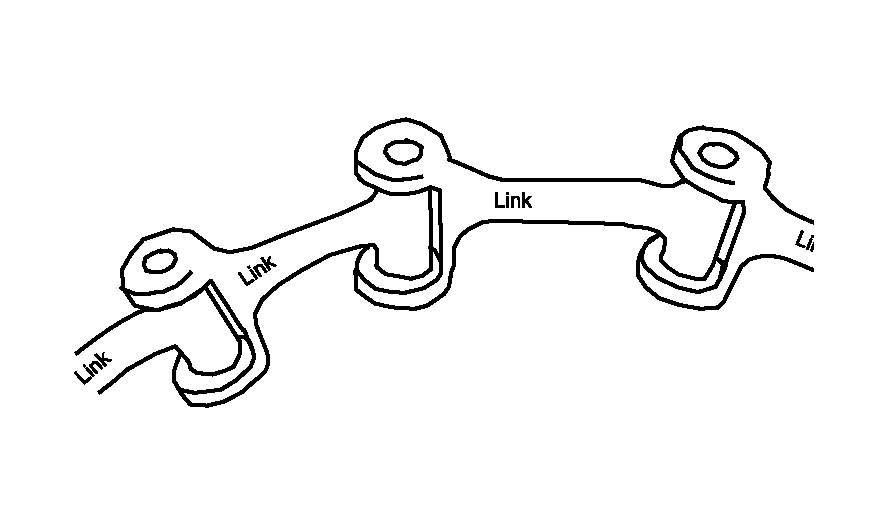
\includegraphics[width=5.0in]{figs03/linkdiag_plain.eps}\\
B)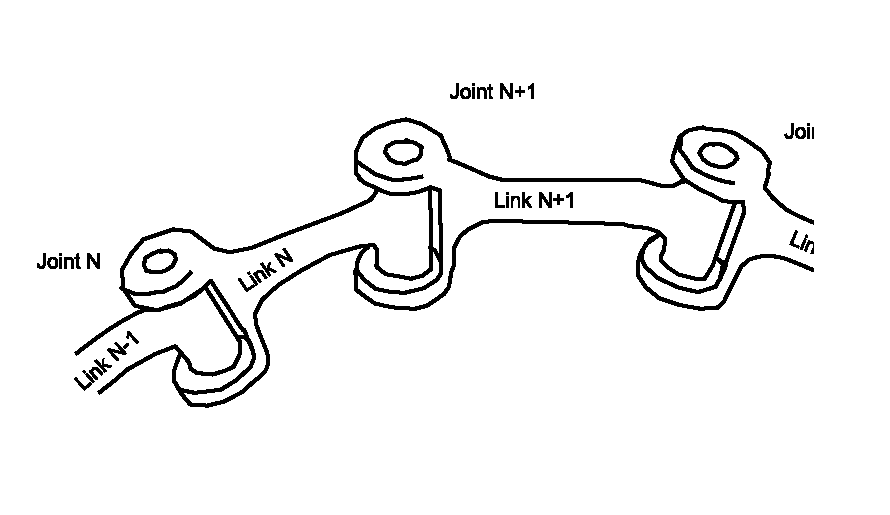
\includegraphics[width=5.0in]{figs03/linkdiag_idlinksjoints.eps}\\
C)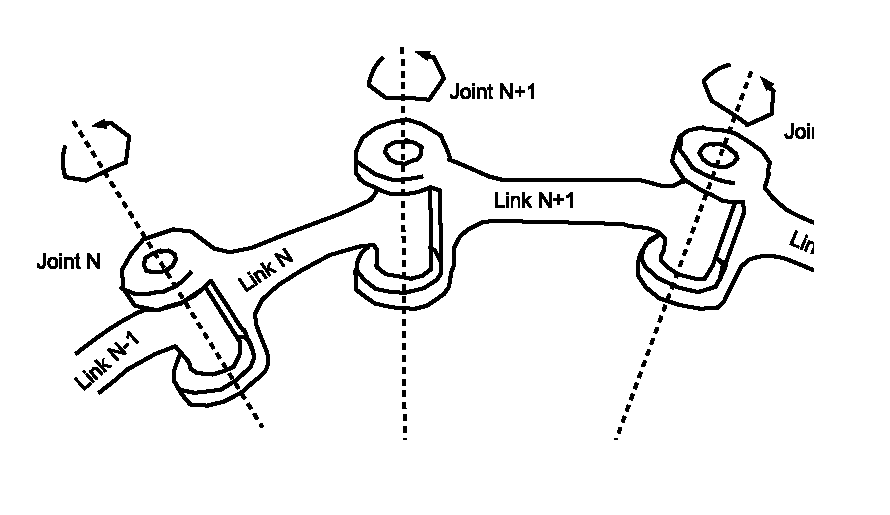
\includegraphics[width=5.0in]{figs03/linkdiag_idaxestypes.eps}
\caption{Summary of steps for analyzing the DH parameters of a serial chain.}\label{DHStepsSummary}
\end{figure}
\begin{figure}[p]
\centering
D)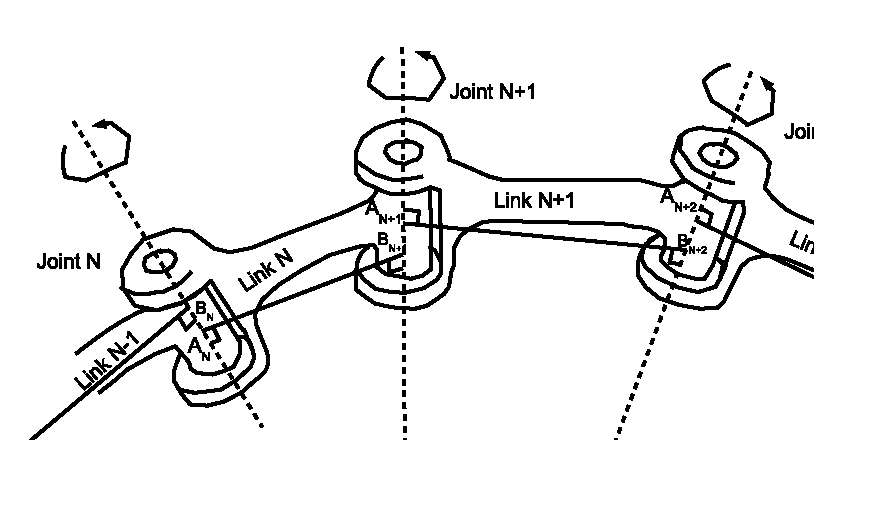
\includegraphics[width=5.0in]{figs03/linkdiag_commonnorms.eps}\\
E)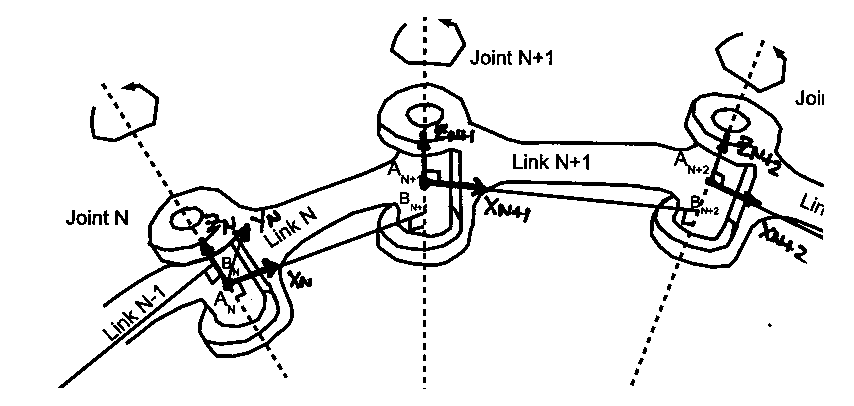
\includegraphics[width=5.0in]{figs03/00336.eps}\\
\caption{Figure \ref{DHStepsSummary} cont.}\label{DHStepsSummary2}
\end{figure}


\clearpage        %  clear floating figures so they appear at next full page



\section{Summary of Link Frame Assignment Methodology}\label{Steps}
We will use the following procedure identify and assign link frames:
\begin{enumerate}
	\item  Understand the geometry and dimensions of the mechanism. Figure \ref{DHStepsSummary}A shows two links (plus parts of two others) of a mechanism we will analyze.


\item Number the links and joints.   The Base of the mechanism is, by convention link 0, and the first joint from the base is numbered joint 1.   In Figure \ref{DHStepsSummary}B we have applied numbers to the links (somewhere in the middle of the chain).




\item  Identify the axes of motion and the directions which you will call positive motion (Figure \ref{DHStepsSummary}C).




\item Draw common normals (CNs) and find their intersections with joint axes.  Define two points on each link:

$A_N$  the intersection of Axis $N$ with the CN to Axis $N+1$.

$B_N$  the intersection of Axis $N$ with the CN to Axis $N-1$.

(Figure \ref{DHStepsSummary}D)


	\item Assign a frame to each link as follows:

The origin of Frame $N$ is $A_N$.

$Z_N$ points along Axis $N$.

$X_N$ points along the CN to $B_{N+1}$

$Y_N$ completes a right handed coordinate system.

(Figure \ref{DHStepsSummary}E)


\end{enumerate}

\vspace{0.25in}


Q:  What if it appears that there is no common normal because the axes intersect?

A: Create a common normal vector with direction but zero length (draw it like a unit vector).
Choose $X_N$ to be normal to $Z_N$ and $Z_{N+1}$.

Q: What if $Z_N$ and $Z_{N+1}$ are parallel and there is no {\it unique} CN?

A: Just choose one of the set of CNs arbitrarily.  Typically you can simplify subsequent analysis by choosing a CN which intersects $B_N$.

Q: What if $Z_N$ and $Z_{N+1}$ are co-linear?

A: Then choose any zero-length vector perpendicular to both of the axes.




%%%%%%%%%%%%%%%%%%%%%%%%%%%%%%%%%%%%%%%%%%%%%%%%%%%%%%%%%%%%%%%%%%%%%%%%
%
%       Example:  Link Frame Assignments, 3 DOF
%
\begin{Example}\label{FKex1}
Assign link frames to the arm shown below.   This arm has two degrees of freedom, but we will define a third frame at the end effector as though the end effector had a degree of freedom attached. The thickness (width) of the arm links is 20cm.


First, we identify the links and joints and number them, starting with link zero and with joint 1 between link zero and link one (blue).
%
% 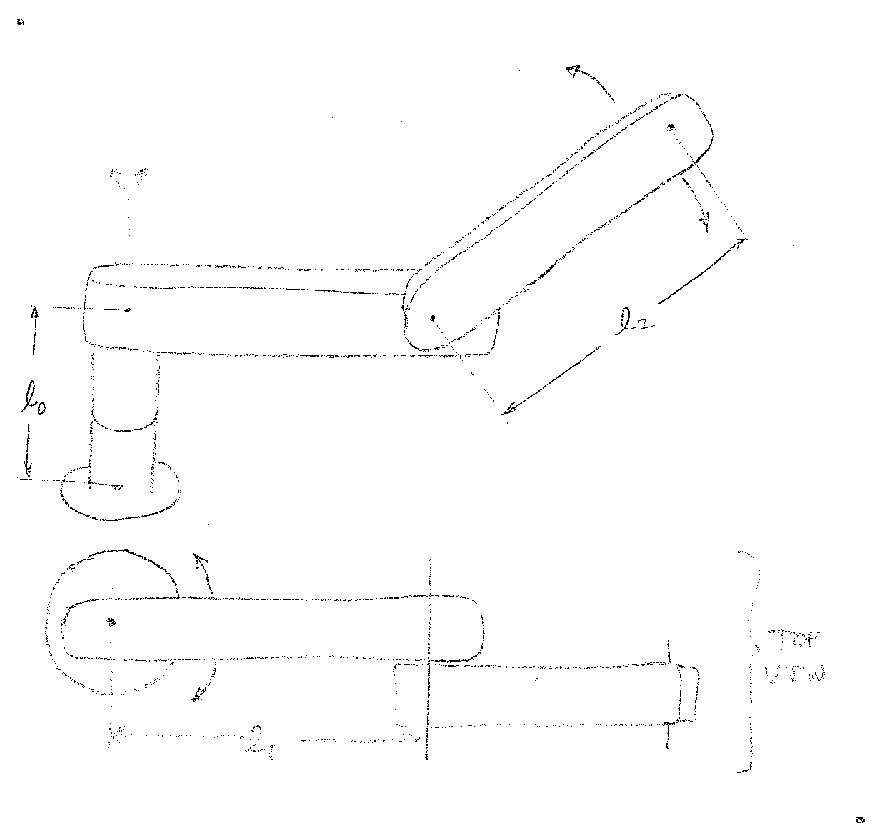
\includegraphics[width=3.25in]{figs03/00408.eps}
%
% \begin{tabular}{cc}
% 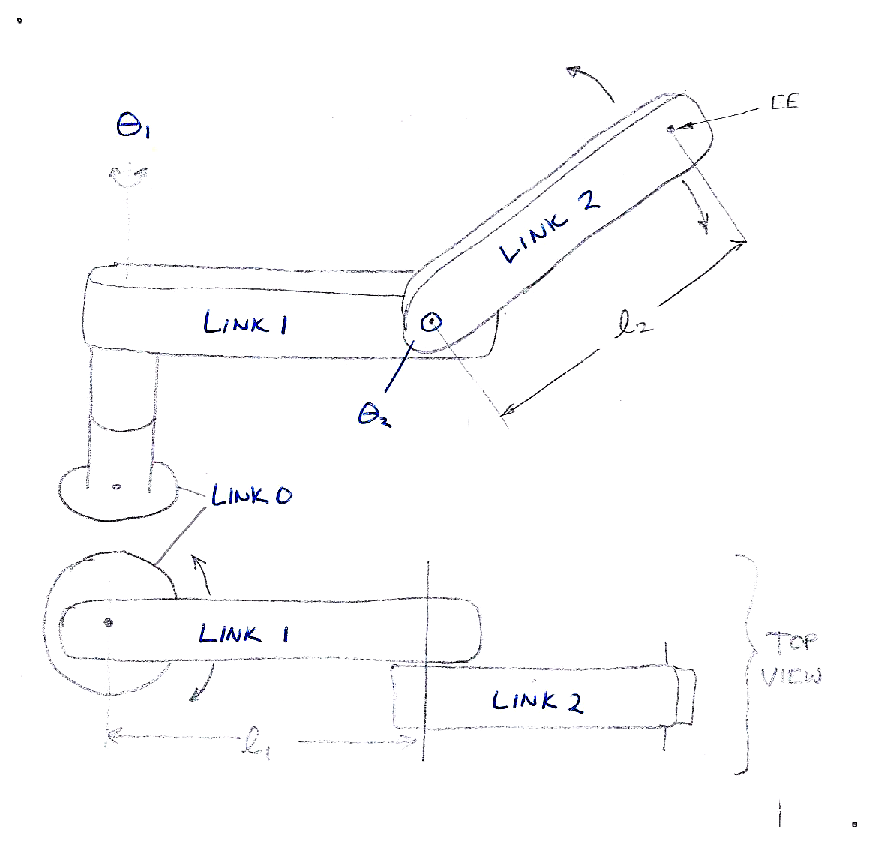
\includegraphics[width=3.25in]{figs03/00409.eps}
% &
% 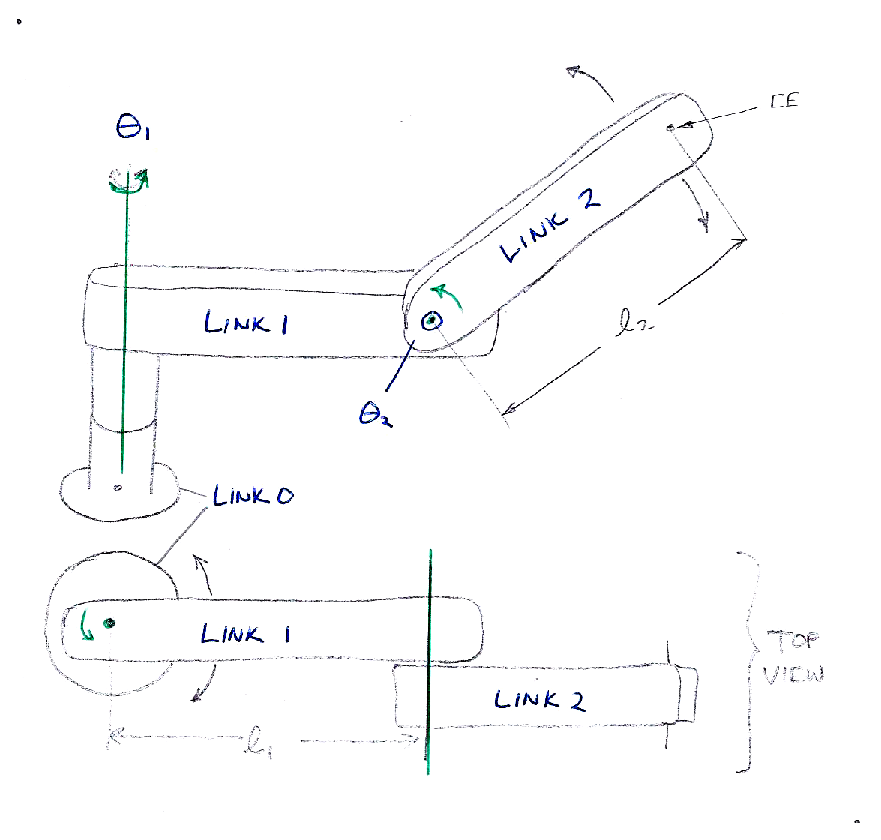
\includegraphics[width=3.25in]{figs03/00410.eps}
% \end{tabular}
% \end{Example}
%
% \begin{ExampleCont}
% \begin{tabular}{cc}
% 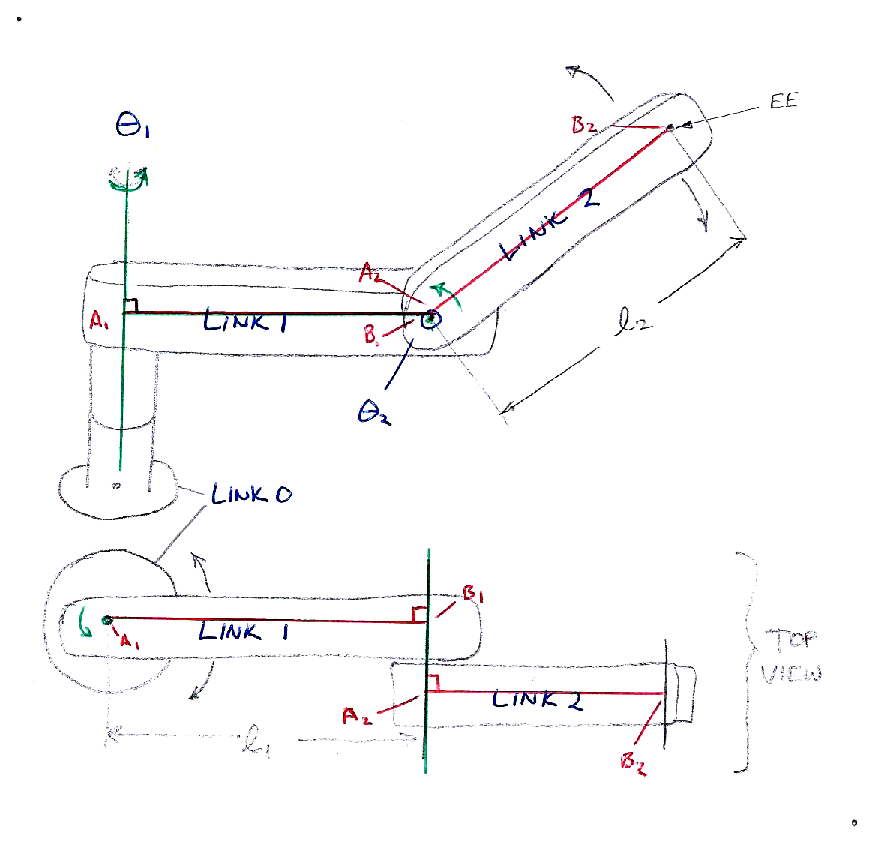
\includegraphics[width=3.25in]{figs03/00411.eps}
% &
% 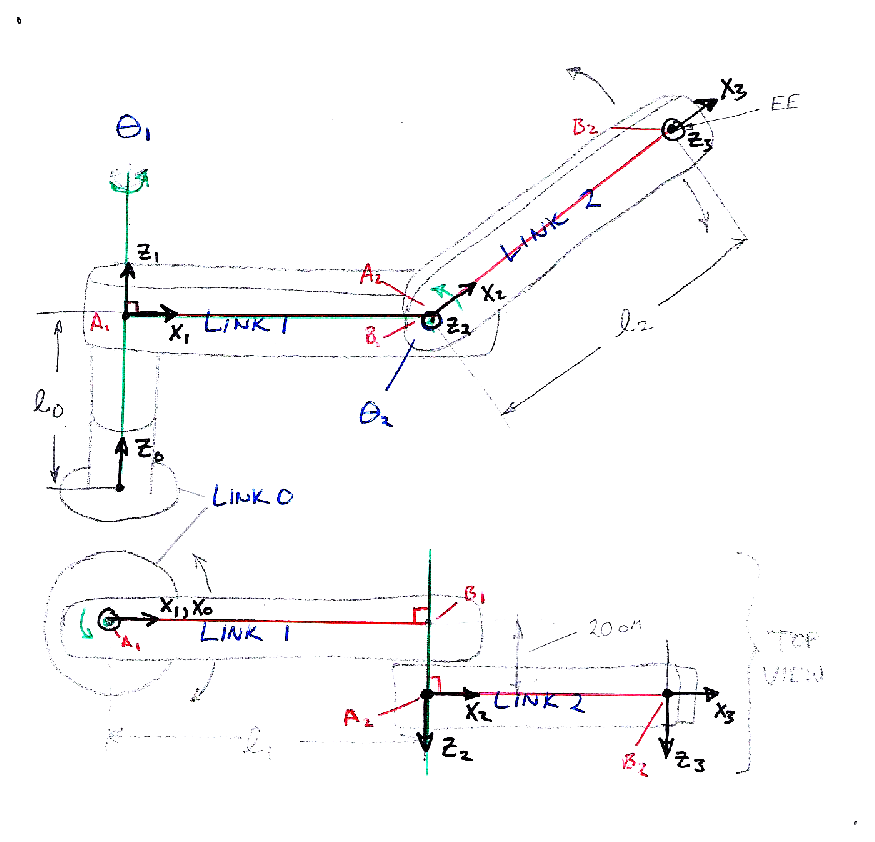
\includegraphics[width=3.25in]{figs03/00412.eps}
% \end{tabular}

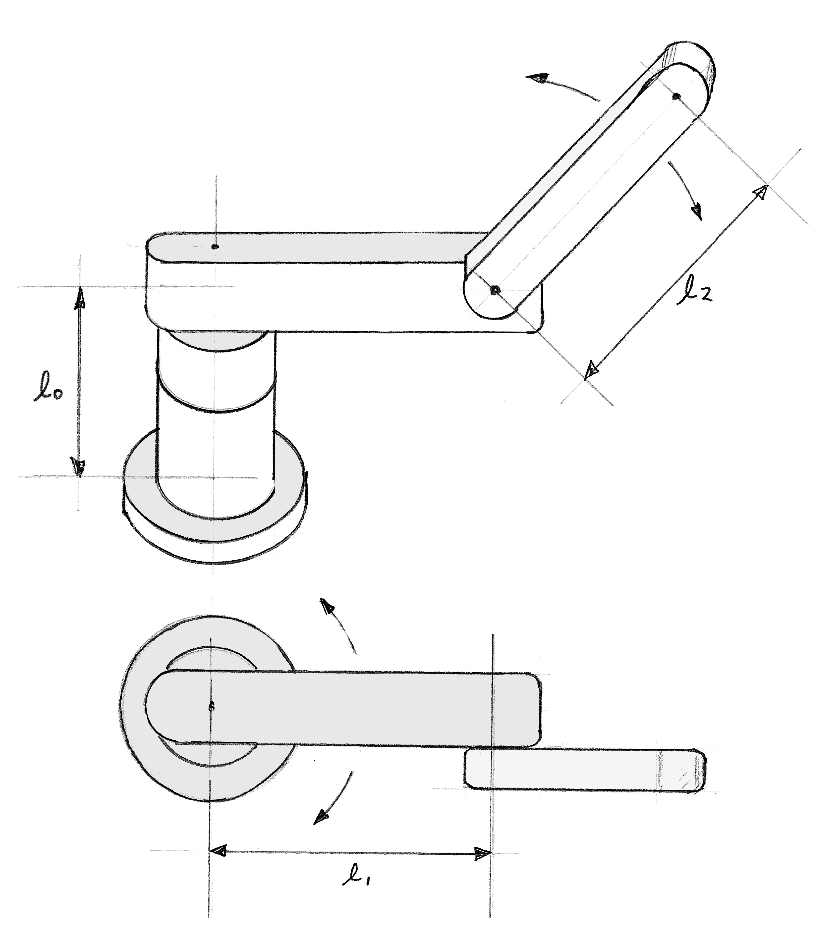
\includegraphics[width=3.25in]{figs03/00715_A.eps}

\begin{tabular}{cc}
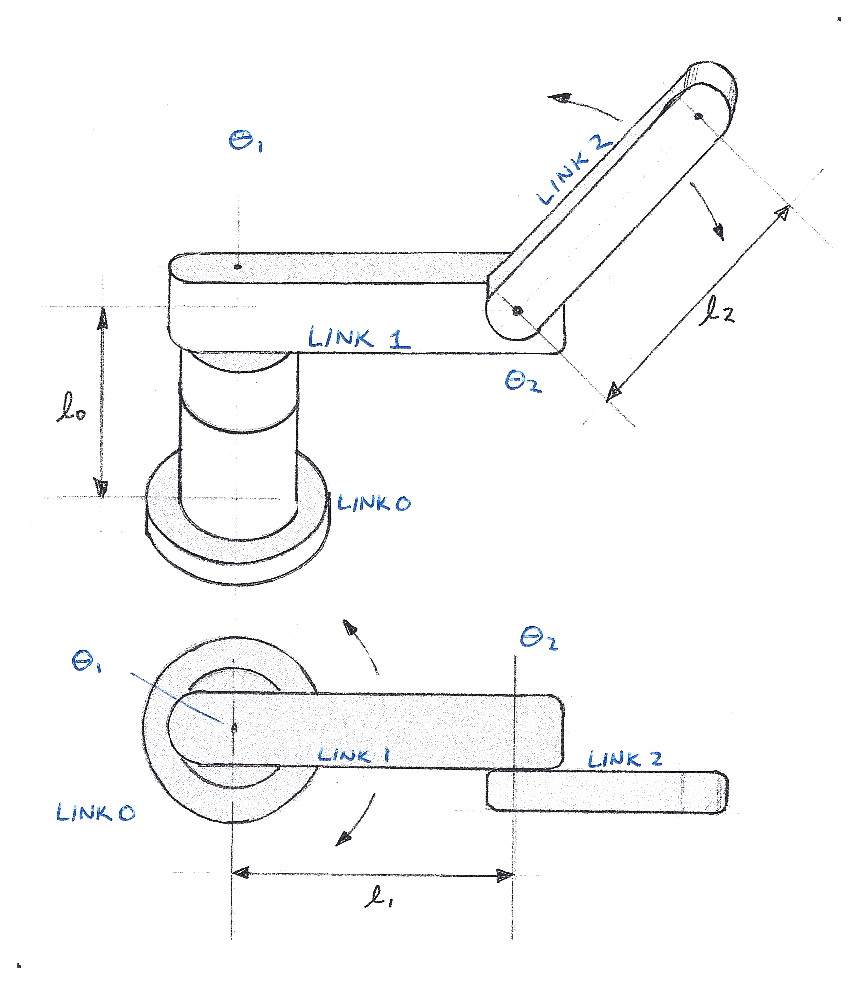
\includegraphics[width=3.25in]{figs03/00715_B.eps}
&
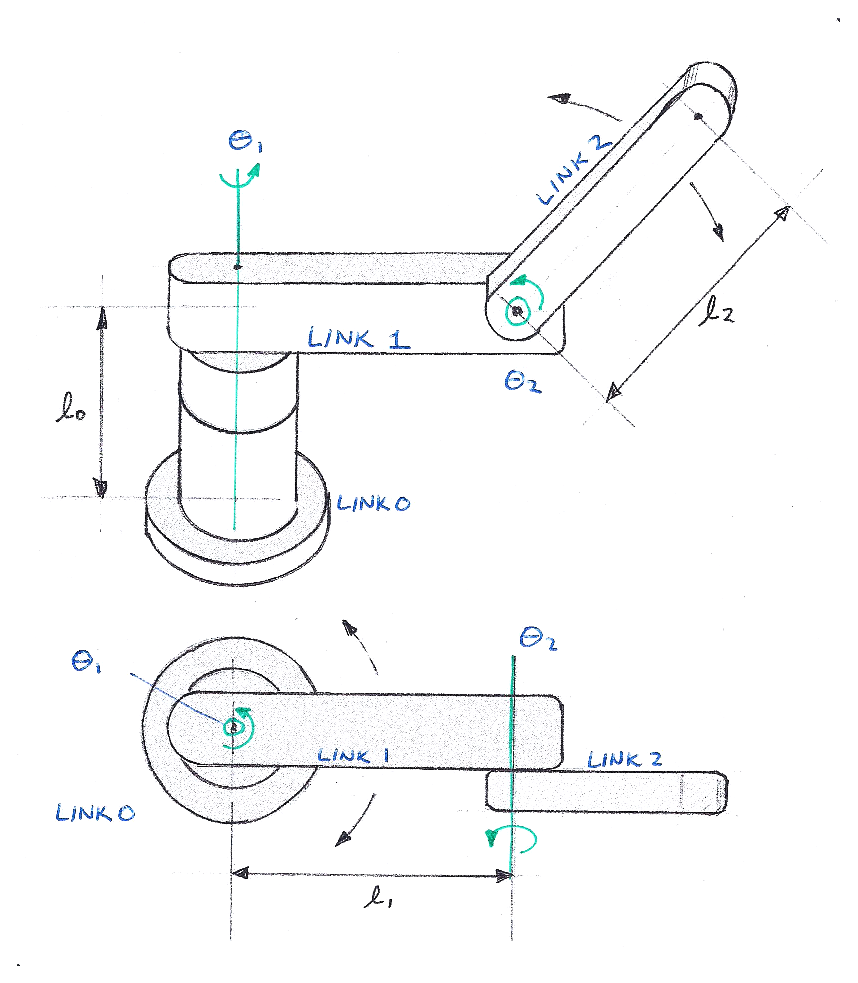
\includegraphics[width=3.25in]{figs03/00715_C.eps}
\end{tabular}
\end{Example}

\begin{ExampleCont}
\begin{tabular}{cc}
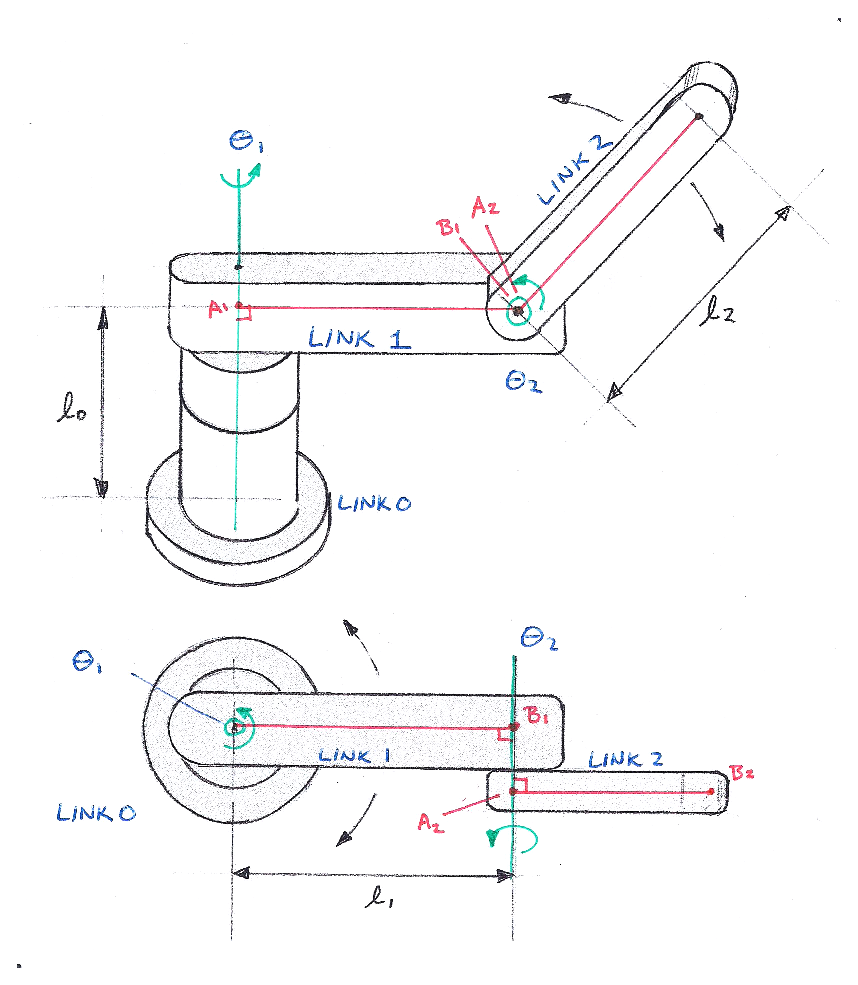
\includegraphics[width=3.25in]{figs03/00715_D.eps}
&
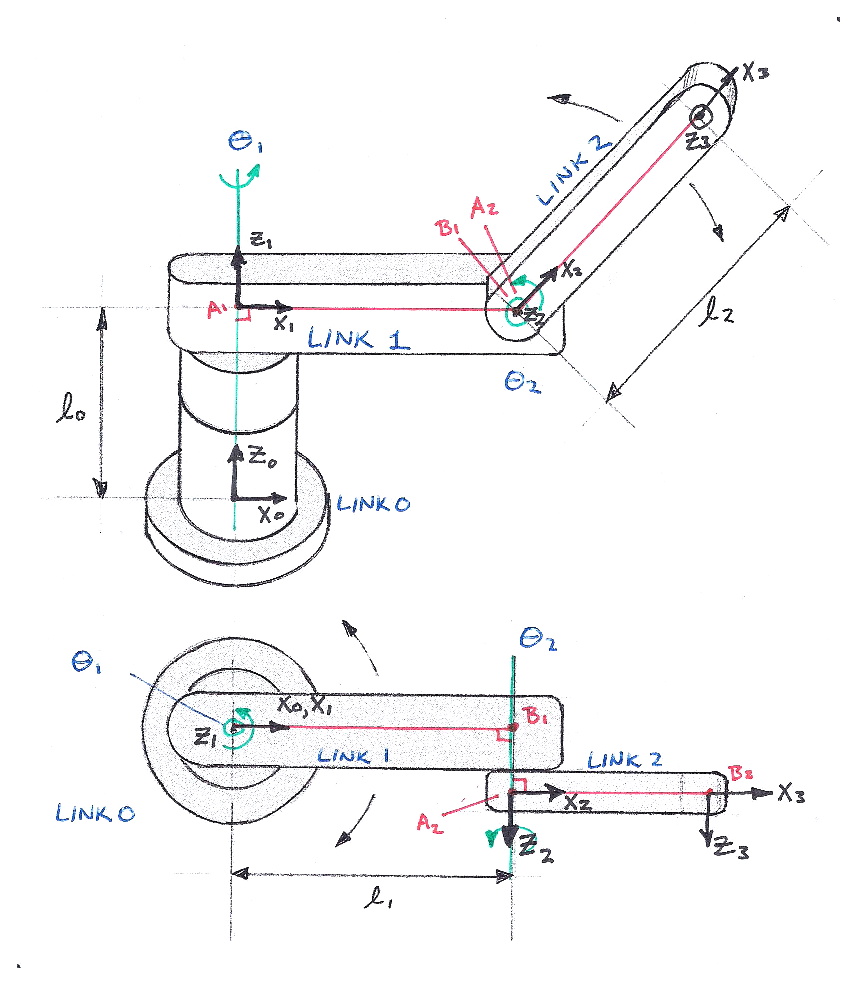
\includegraphics[width=3.25in]{figs03/00715_E.eps}
\end{tabular}


Second we identify the joint axis lines and choose directions of rotation around them (for rotary joints) which we denote to be positive (green).

Third, we draw in the common normals between the identified joint axes (red).

Finally, we identify the origins of each link frame, draw in $z_i$ pointing so that positive rotation follows the RHR, and draw $x_i$ along the common normal to the next axis (black).

A simplified stick figure (below) can sometimes help in visualizing the frame assignments:

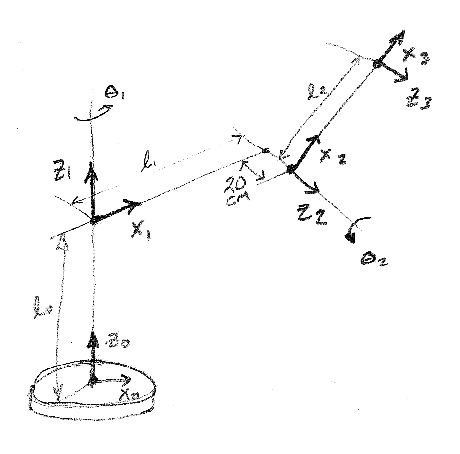
\includegraphics[width=72mm]{figs03/00885.eps}

\end{ExampleCont}
%%%%%%%%%%%%%%%%%%%%%%%%%%%%%%%%%%%%%%%%%%%%%%%%%%%%%%%%%%%%%%%%%%%%%%%%%%%%%%%%%%%%%%
%%%%%%%%%%%%%%%%%%%%%%%%%%%%%%%%%%%%%%%%%%%%%%%%%%%%%%%%%%%%%%%%%%%%%%%%
%
%       Example:  Link Frame Assignments: 6 DOF:   Stanford Arm
%
\begin{Example}

This example considers the 6 DOF arm designed by Vic Scheinman and Bernard Roth, the ``Stanford Arm".   The series of four drawings shows the steps in analyzing and applying frames to the arm.   Following the steps above in Section \ref{Steps}.

1) Understand the geometry and dimensions of the mechanism.  The first drawing indicates only the shape and motions of the arm.

2) In step two we number the links and joints.  It turns out that numbering the Joints is most important and we skip explicitly numbering the joints here. We add some dimensions for the shoulder height, $L_1$ and the shoulder offset $S$.

3) In green in the second drawing,  we highlight the directions we will consider positive motion,

4) This arm features all intersecting axes (to simplify the equations).  In drawing 3, we show in red CN vectors obtained by crossing sequential axes.

5) In drawing 4 we assign a link frame to each axis according to Step 5 of Section \ref{Steps}.

1) 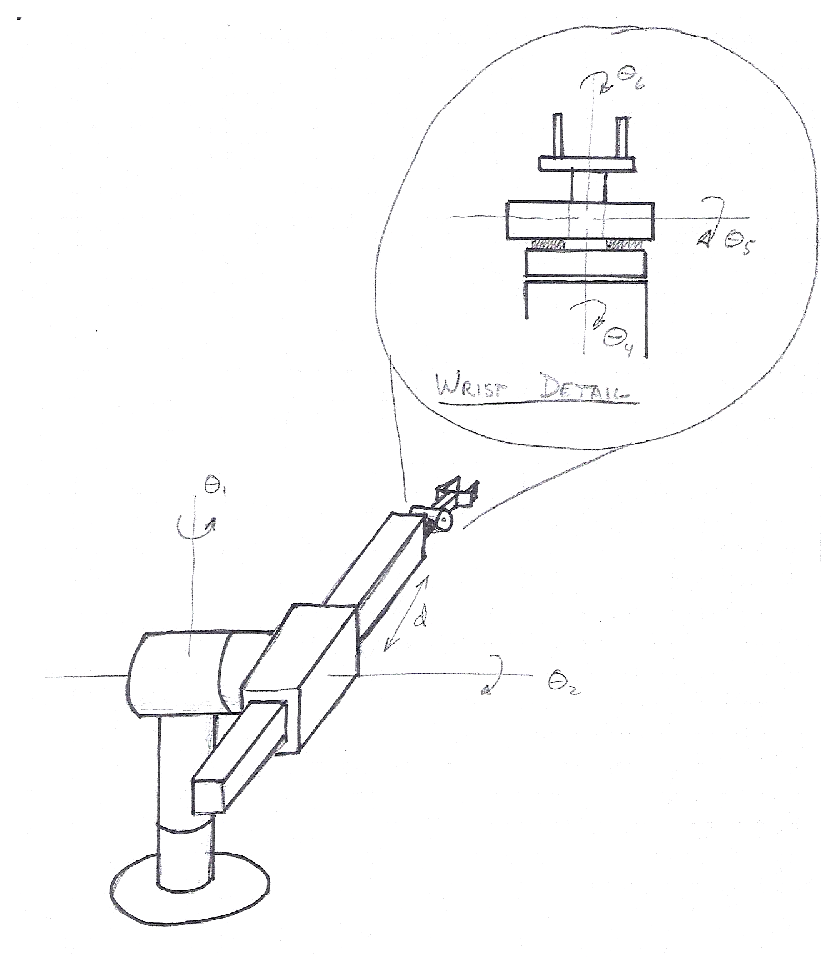
\includegraphics[width=3.2in]{figs03/00416.eps}
2) 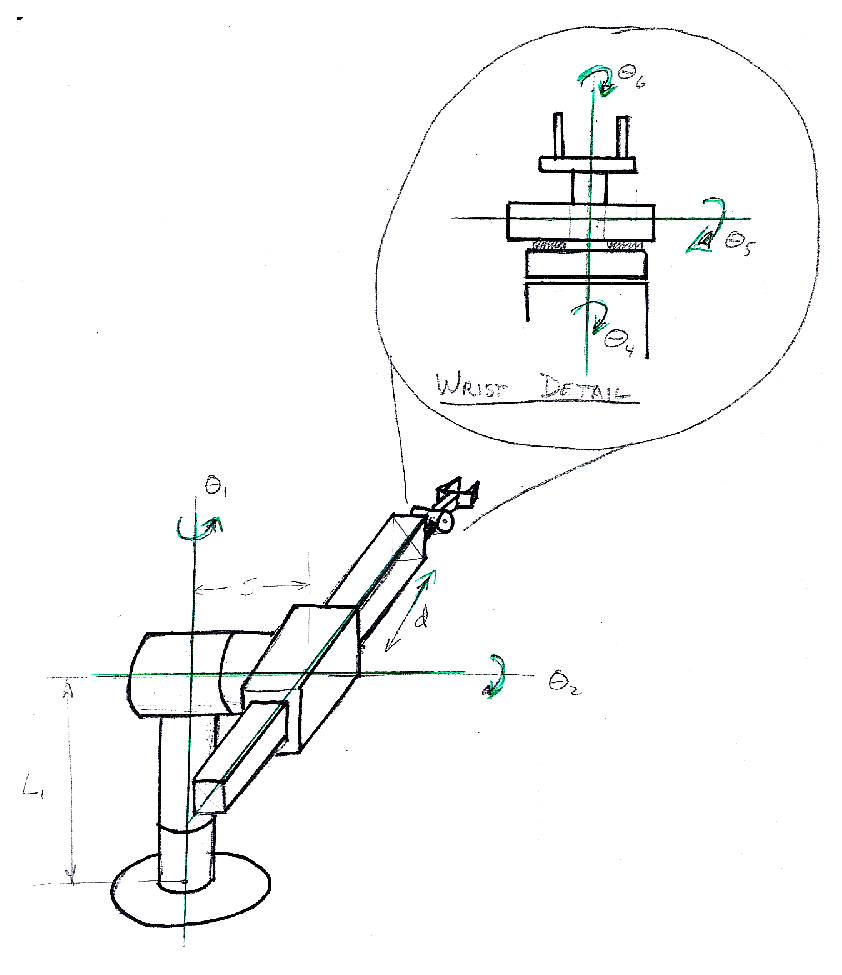
\includegraphics[width=3.2in]{figs03/00417.eps}\\
3) 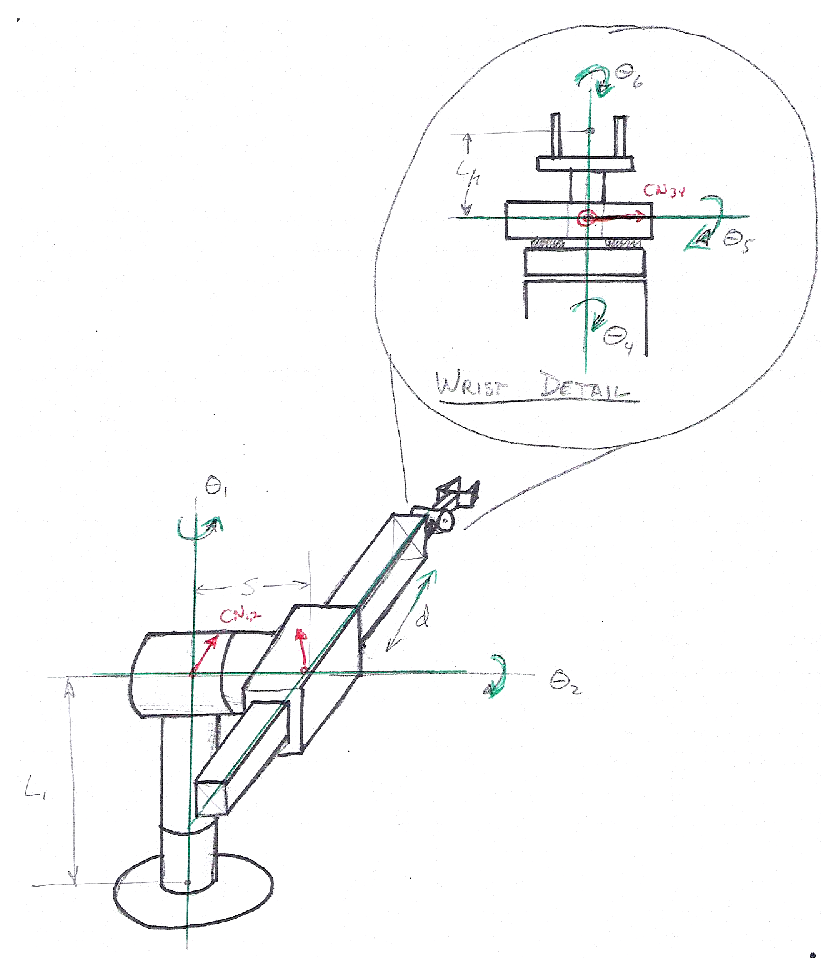
\includegraphics[width=3.2in]{figs03/00418.eps}
4) 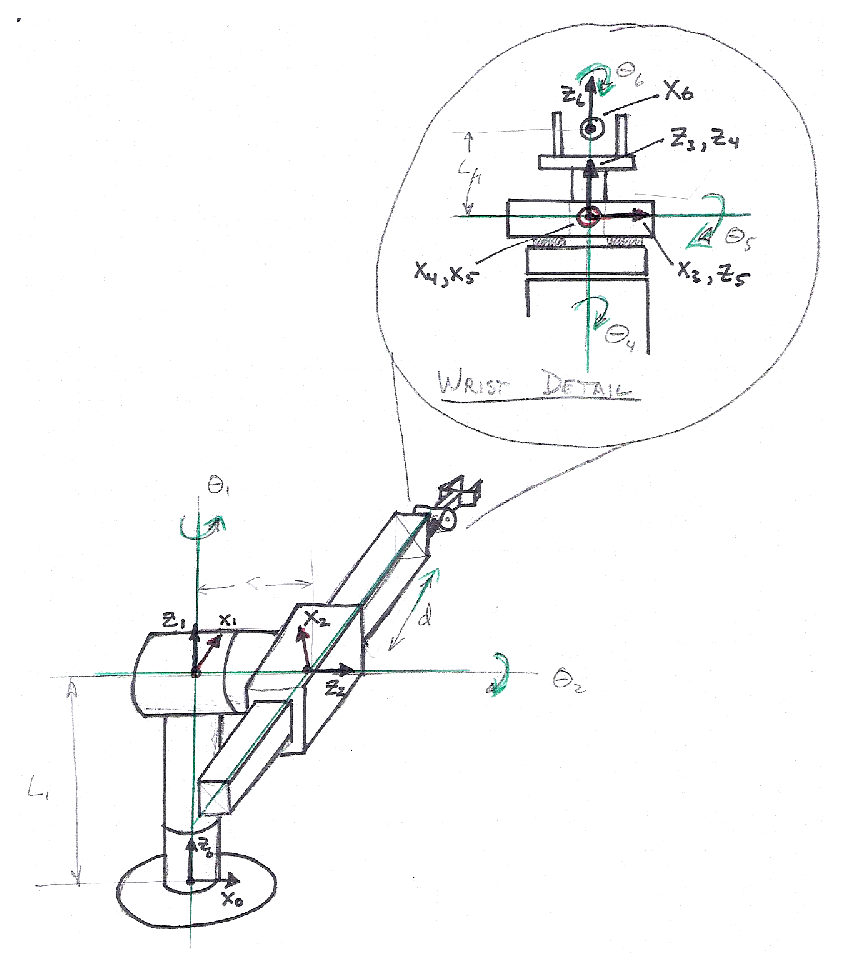
\includegraphics[width=3.2in]{figs03/00419.eps}

\label{FKex2}
\end{Example}



\section{Denavit Hartenberg Parameters}

In 1955 Denavit and Hartenburg created a standardized way to derive transforms from one link to another in a serial chain.  Once frames have been assigned to each link as described above, for each link, we will be able to identify two specific rotations and two translations which uniquely define the relationship between the links.  Of the four Denavit-Hartenberg (DH) parameters, three are fixed constants due to the rigid body nature of the link.  A fourth is a variable which specifies the relative motion between the link and the next link.  For rotary joints that variable is $\theta_N$ and for prismatic joints, that variable is $d_N$.  The definition of the four DH parameters are now given.    A very nice video illustration of the DH parameters is available at the wikipedia page for ``Denavit-Hartenberg Parameters".

\subsubsection{Composition of parameters}

\begin{figure}\centering
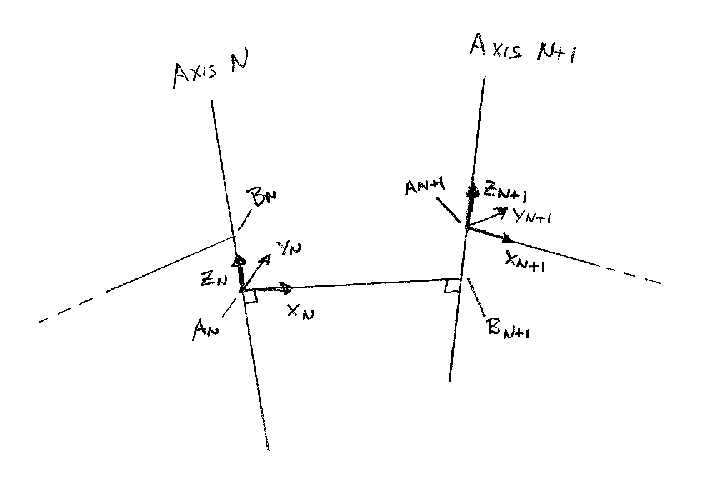
\includegraphics[width=3.5in]{figs03/00340.eps}
\caption{Virtual links with link frames fixed in both position and orientation.}\label{VirtualLinkswFrames}
\end{figure}

We use the DH parameters to describe the spatial relationship between frame $N-1$ and frame $N$.    Notice that a series of axes and CNs forms a continuous path from one link frame origin to the next.    We will follow this path through its twists and turns and describe each translation and rotation with a single DH parameter.  Each DH parameter represents a rotation or a translation about a single known axis.   Since the origin of Frame $N-1$ is $A_{N-1}$ we start there  and work our way to the origin of the next frame.   Refering to Figure \ref{VirtualLinkswFrames}, we rotate by the {\bf link twist}:  $\mathrm{Rot}(\hat{x},\alpha_{N-1})$, then translate by the {\bf link length}: Trans$(\hat{x},a_{N-1})$, then rotate by the {\bf joint angle}: Rot$(\hat{z}, \theta_N)$, and finally translate by the {\bf joint offset}: Trans$(\hat{z}, d_N)$.   Note that the relationship between link $N-1$ and link $N$ is described by parameters with a mix of subscripts.   The Denavit Hartenberg parameters can be visualized in
Figure \ref{CraigPaulLinkFrames}.

For the common case of rotary joints,  $a_{N-1}, \alpha_{N-1}, d_N$ will be fixed constants, dependent on the geometric design of the arm, and $\theta_N$ will be a variable joint angle.   Some arms include prismatic joints in which $\theta_N$ is a constant and $d_N$ is a variable.   In evaluating the link transform we typically replace all constant parameters with their measured or design values and keep the single variable parameter in DH form.     In rare cases, a joint includes two degrees of freedom such as a cylindrical shaft which can rotate as well as translate\footnote{See for example, the last two degrees of freedom of the SCARA arm.}.   In this case it is best to abstract that joint into two separate joints, one for rotation and one for translation.

Our strategy will be to multiply together 4x4 homogeneous transforms for each of the elemental displacement and rotations above which make up the virutal link.   To keep the notation under control we will use the following shorthand:

\[
 c\theta_j \equiv c_j \equiv cos(\theta_j)
\]
\[
s\theta_j \equiv s_j \equiv sin(\theta_j)
\]


The complete transform is then
\[
^{N-1}_NT =  \mathrm{Rot}(\hat{x},\alpha_{N-1})\mathrm{Trans}(\hat{x},a_{N-1})\mathrm{Rot}(\hat{z}, \theta_N)\mathrm{Trans}(\hat{z}, d_N)
\]
or equivalently

\[
^{N-1}_NT =  \mathrm{Rot}(\hat{x},\alpha_{N-1})\mathrm{Trans}(\hat{x},a_{N-1})\mathrm{Rot}(\hat{z}, \theta_N)\mathrm{Trans}(\hat{z}, d_N)
\]

\[
= \left[
   \begin{array}{cccc}
    1     &     0     &     0     &      0   \\
    0     &     c\alpha_{N-1}     &     -s\alpha_{N-1}     &      0   \\
    0     &     s\alpha_{N-1}     &      c\alpha_{N-1}     &      0   \\
    0     &     0     &     0     &      1   \\
   \end{array}
  \right ]
   \left[
   \begin{array}{cccc}
    1     &     0     &     0     &      a_{N-1}   \\
    0     &     1     &     0     &      0   \\
    0     &     0     &     1     &      0   \\
    0     &     0     &     0     &      1   \\
   \end{array}
  \right ]
   \left[
   \begin{array}{cccc}
    c\theta_N     &     -s\theta_N    &     0     &      0   \\
    s\theta_N     &      c\theta_N    &     0     &      0   \\
    0     &     0     &     1     &      0   \\
    0     &     0     &     0     &      1   \\
   \end{array}
  \right ]
   \left[
   \begin{array}{cccc}
    1     &     0     &     0     &      0   \\
    0     &     1     &     0     &      0   \\
    0     &     0     &     1     &      d_N   \\
    0     &     0     &     0     &      1   \\
   \end{array}
  \right ]
  \]


or equivalently

\[
^{N}_{N+1}T =  \mathrm{Rot}(\hat{x},\alpha_{N})\mathrm{Trans}(\hat{x},a_{N})\mathrm{Rot}(\hat{z}, \theta_{N+1})\mathrm{Trans}(\hat{z}, d_{N+1})
\]

\[
= \left[
   \begin{array}{cccc}
    1     &     0     &     0     &      0   \\
    0     &     c\alpha_{N}     &     -s\alpha_{N}     &      0   \\
    0     &     s\alpha_{N}     &      c\alpha_{N}     &      0   \\
    0     &     0     &     0     &      1   \\
   \end{array}
  \right ]
   \left[
   \begin{array}{cccc}
    1     &     0     &     0     &      a_{N}   \\
    0     &     1     &     0     &      0   \\
    0     &     0     &     1     &      0   \\
    0     &     0     &     0     &      1   \\
   \end{array}
  \right ]
   \left[
   \begin{array}{cccc}
    c\theta_{N+1}     &     -s\theta_{N+1}    &     0     &      0   \\
    s\theta_{N+1}     &      c\theta_{N+1}    &     0     &      0   \\
    0     &     0     &     1     &      0   \\
    0     &     0     &     0     &      1   \\
   \end{array}
  \right ]
   \left[
   \begin{array}{cccc}
    1     &     0     &     0     &      0   \\
    0     &     1     &     0     &      0   \\
    0     &     0     &     1     &      d_{N+1}   \\
    0     &     0     &     0     &      1   \\
   \end{array}
  \right ]
  \]

Each of these four matrices is a function of one of the four DH parameters.   We can then multiply them together to get a single matrix which represents the link.

\subsubsection{Generalized Link Transformation}
By multiplying all four matrices together we get the following transform for any link which has DH parameters:
\begin{equation}\label{DHLinkTransform}
^{N-1}_NT = \left [
  \begin{array}{cccc}
  c\theta_N	          & -s\theta_N	             &     0         &   a_{N-1}	\\
  s\theta_Nc\alpha_{N-1}  &  c\theta_Nc\alpha_{N-1}  & -s\alpha_{N-1}  & -s\alpha_{N-1}d_N  \\
  s\theta_Ns\alpha_{N-1}  & c\theta_Ns\alpha_{N-1}   & c\alpha_{N-1}   & c\alpha_{N-1}d_N  \\
   0 & 0 & 0 & 1
  \end{array}
\right ]
\end{equation}

The reader can derive the corresponding matrix for $^{N}_{N+1}T$.


\subsection{Combining links into a chain}

Once we have $^{N-1}_NT$ for all of the links, we multiply them together to get the full forward kinematics model. For example in a three link robot we would have
\[
^0_3T = \;^0_1T \;^1_2T \;^2_3T
\]

Usually it is possible and desirable to multiply them together in symbolic form.    We will bring this process together in the next section.

\subsection{Summary of Forward Kinematics Analysis Part 2}\label{DH_Steps}
\begin{enumerate}
\item Derive the Denavit Hartenberg parameters, $a_N, \alpha_N, d_N, \theta_N,$ from your assigned link frames as follows:

$a_N$ is the distance from $A_N$ to $B_{N+1}$.  This is the distance along the CN from $Z_N$ to $Z_{N+1}$.  $a_N$ is refered to as the ``link length" (see Figure \ref{VirtualLinksCN} and Figure \ref{DHStepsSummary2} D and E).

$\alpha_N$ is the angle between Axis $N$ and Axis $N+1$ about the common normal.  This is the angle between $Z_N$ and $Z_{N+1}$ about $X_N$ in the RHR sense.   $\alpha_N$ is called the ``link twist".

$d_N$ is the distance from $B_N$ to $A_N$.   This is the distance from $X_{N-1}$ to $X_N$ along $Z_N$.   $d_N$ is referred to as the ``joint offset".

$\theta_N$ is the angle between CN$_{N-1}$ and CN$_{N}$ around Axis $N$.  This is the angle between $X_{N-1}$ and $X_N$ around $Z_N$.   $\theta_N$ is refered to as the ``joint angle".

\item Use equation \ref{DHLinkTransform} to compute the link transform for each link


\item Multiply all the link transforms together.

\end{enumerate}





%%%%%%%%%%%%%%%%%%%%%%%%%%%%%%%%%%%%%%%%%%%%%%%%%%%%%%%%%%%%%%%%%%%%%%%%
%
%       Example:  DH parameters and Link Transforms: 3DOF
%
\begin{Example}
Find the 4x4 matrix representing the forward kinematic equations of the manipulator of Example \thechapter.\ref{FKex1}.
\vspace{0.075in}

Step 1.  Referring to the procedure of Section \ref{DH_Steps}

\begin{tabular}{|c|c|c|c|c|} \hline
$N$	&  $\alpha_{N-1}$   &  $a_{N-1}$    	& $d_N$		&  $\theta_N$  	\\ \hline
1	&     0        &     0			&  $l_0$	&  $\theta_1$  	\\ \hline
2	&   $90^{\circ}$	& $l_1$	&  20cm		&  $\theta_2$  		\\ \hline
3	&   0	&    $l_2$ 			&  0		&    0         	\\ \hline
\end{tabular}

\vspace{0.075in}

Step 2

Referring to Equation \ref{DHLinkTransform}

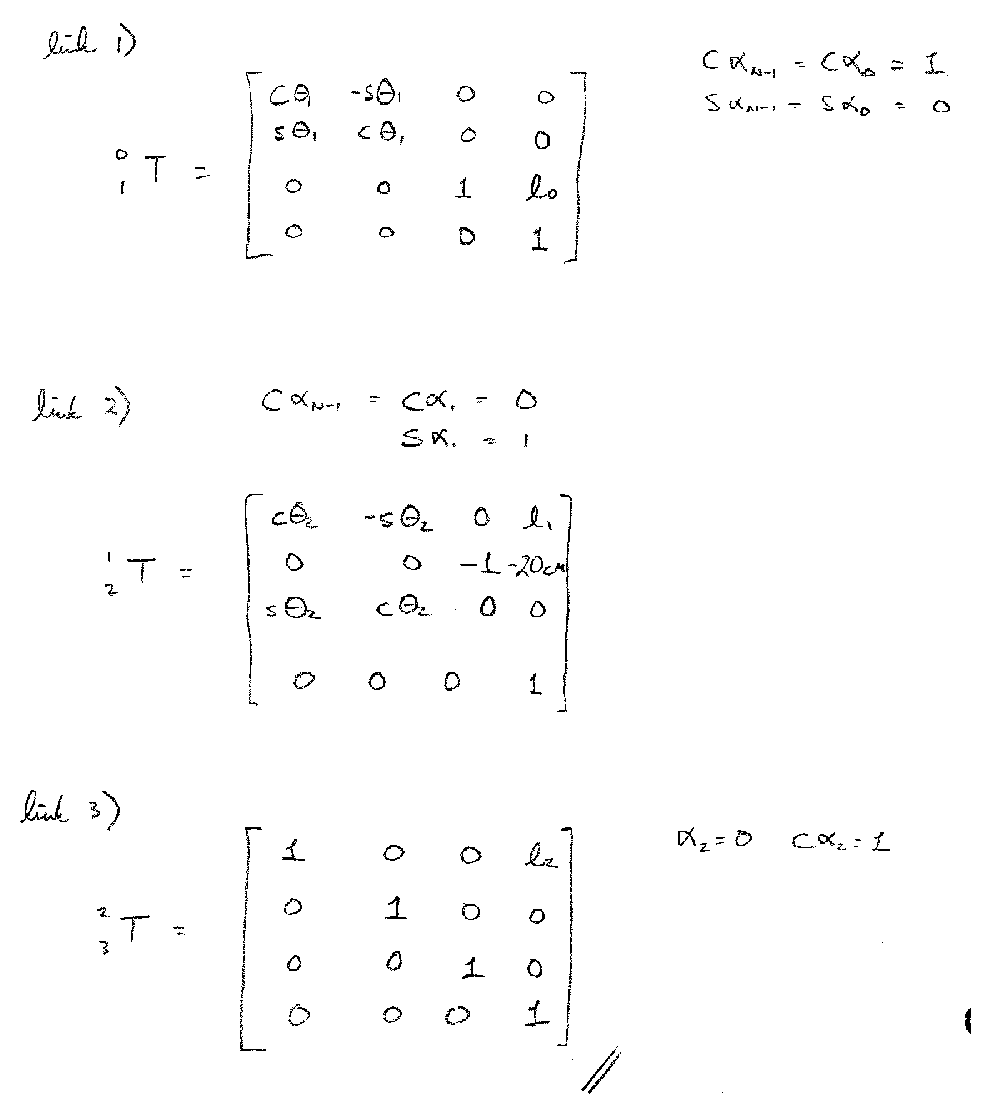
\includegraphics[width=5.0in]{figs03/00413.eps}
\end{Example}

\begin{ExampleCont}
Step 3

Now multiplying the three matrices together we get:

\includegraphics[width=5.0in]{figs03/00414.eps}

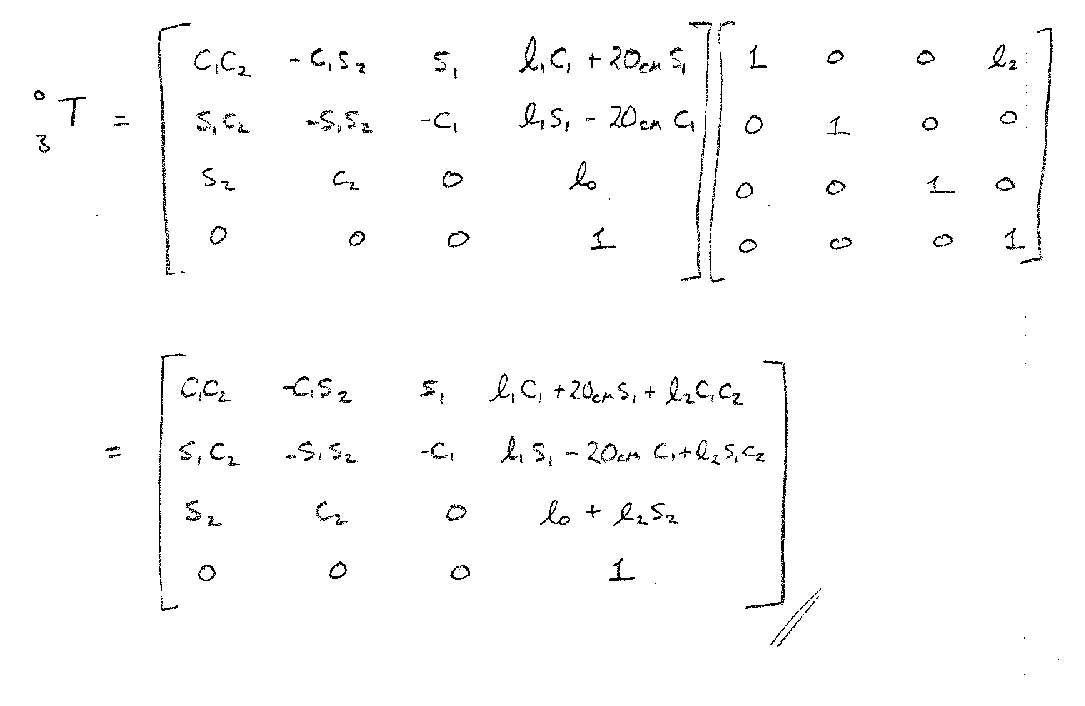
\includegraphics[width=5.0in]{figs03/00415.eps}

\end{ExampleCont}
%%%%%%%%%%%%%%%%%%%%%%%%%%%%%%%%%%%%%%%%%%%%%%%%%%%%%%%%%%%%%%%%%%%%%%%%%%


\begin{Example}
Find link frame assignments and Denavit Hartenberg parameters for the Rosheim Prehensile Wrist\footnote{Mark Rosheim, ``Robotic Wrist Actuators,''  John Wiley \& Sons, 1989.}.   The following interesting wrist mechanism has an extraordinary range of pitch orientations.

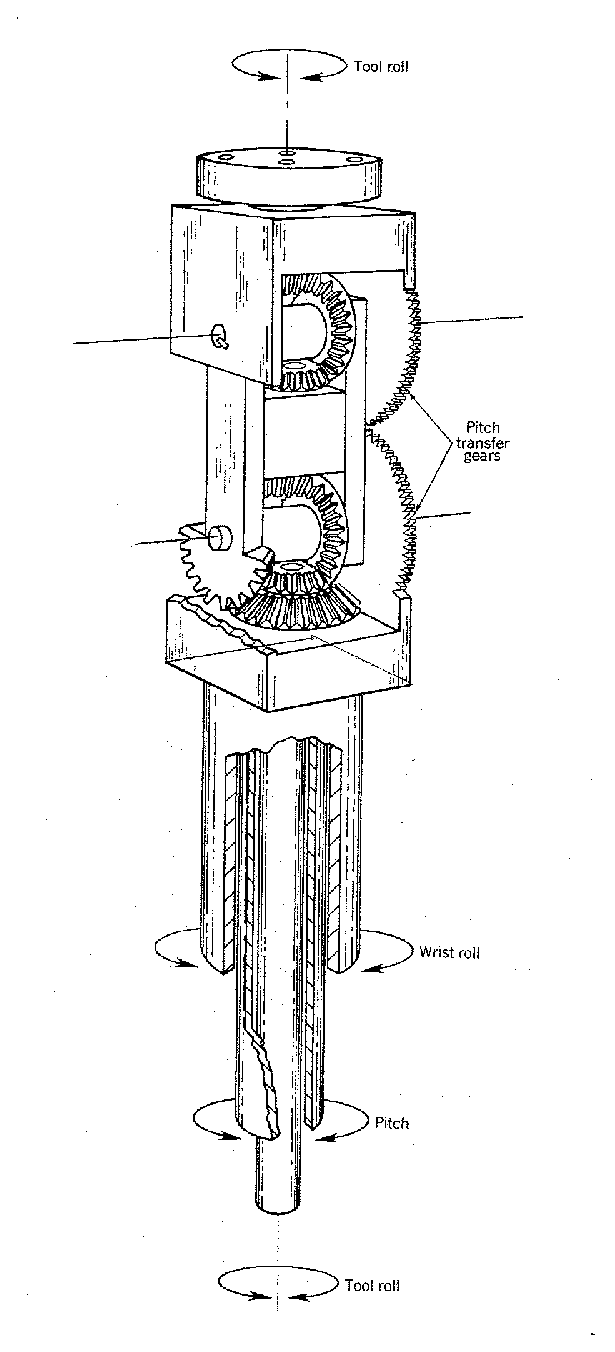
\includegraphics[width=5cm]{figs03/00420.eps}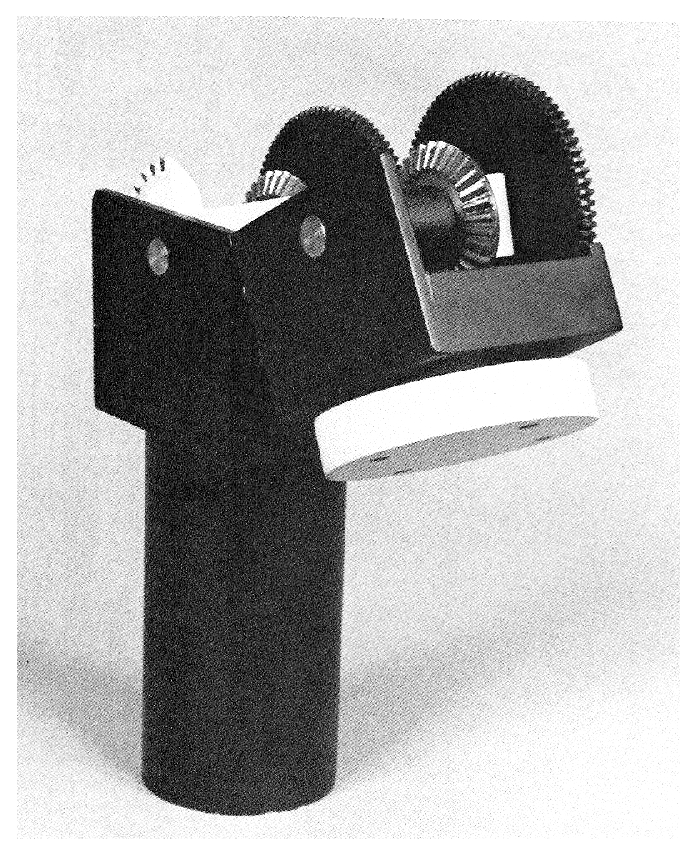
\includegraphics[width=7.5cm]{figs03/rosheim_pre_photo.eps}

\end{Example}

\newpage
\begin{ExampleCont}
Following the steps outlined above:

1) Understand the geometry and dimensions.   First, we arbitrarily identify the bottom of the rectanglar solid below the first bevel gears as a reference plane (i.e. we will locate Frame 0 there in the next step).  We draw diagonals in that plane to locate its center.  We also extend the joint axis lines through the joints and give names to the dimentions between them:



2) Number the Links and Joints.   Furthermore, the Wrist roll axis intersects the first horizontal axis (which we will call joint 2 in the next step) so that link 1 has zero length:

1) 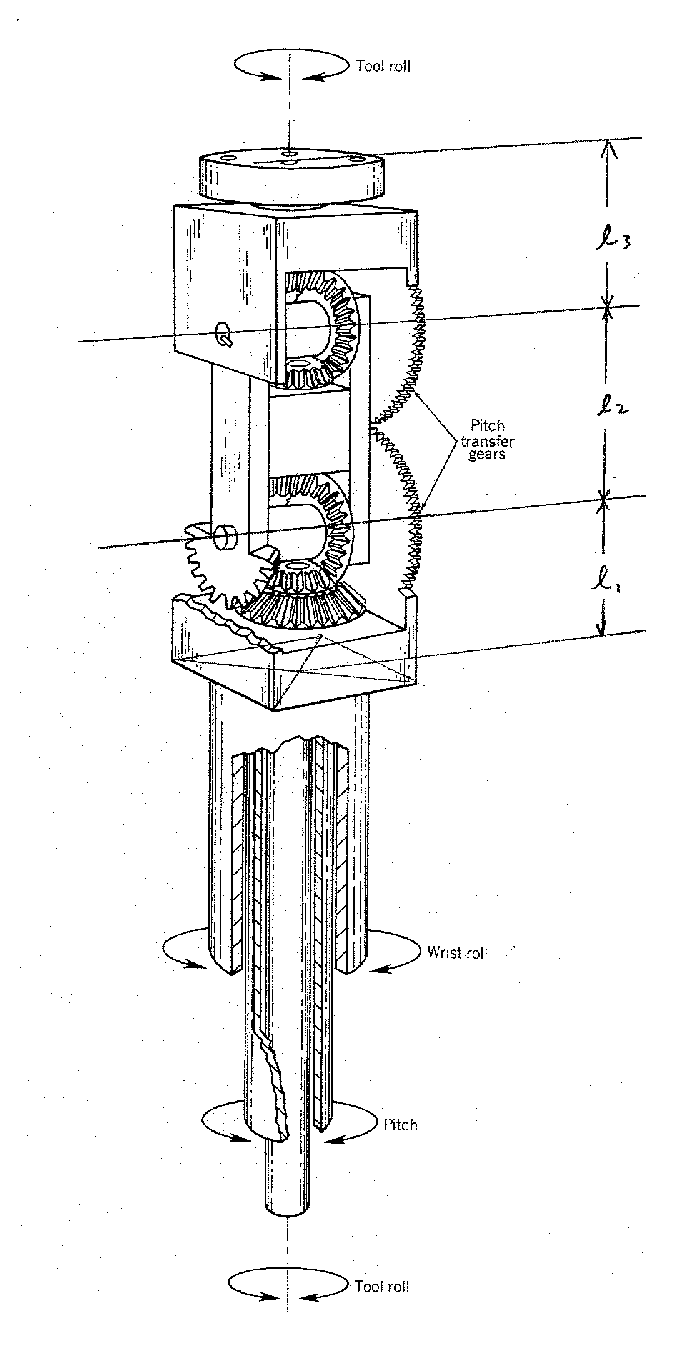
\includegraphics[width=5.38cm]{figs03/00421.eps} 2) 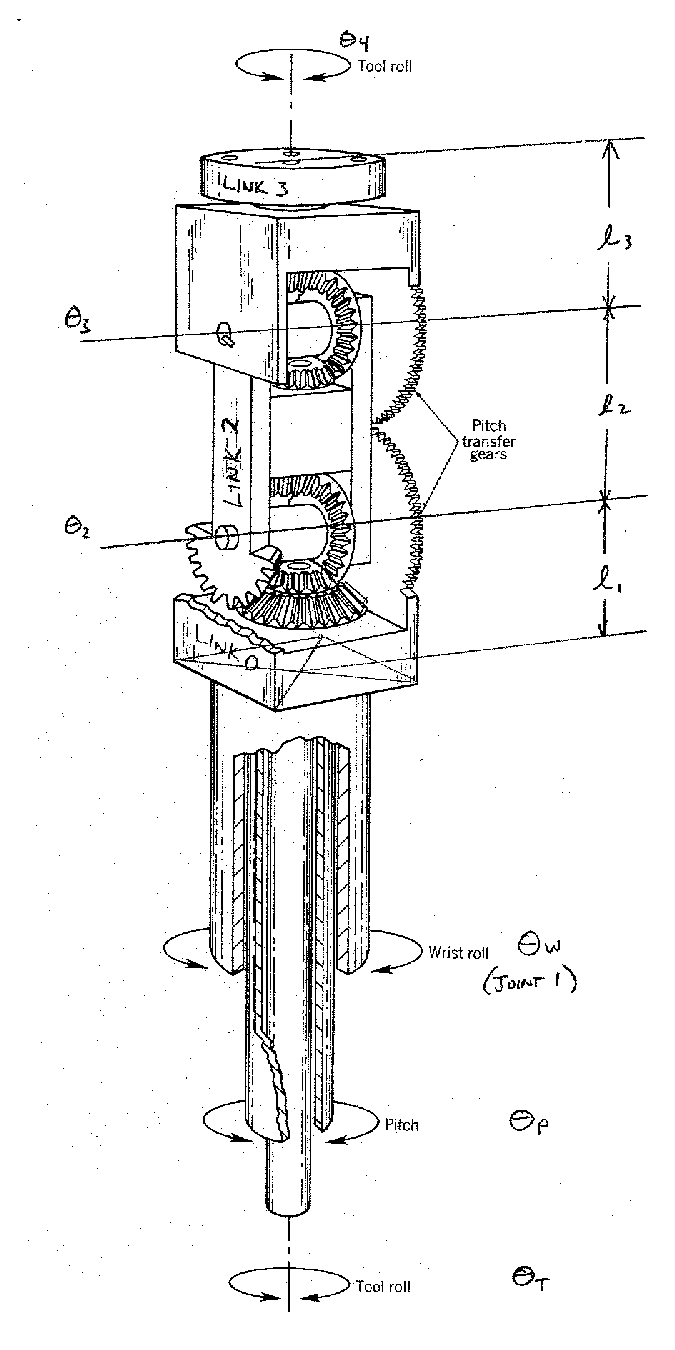
\includegraphics[width=5.38cm]{figs03/00422.eps}

\end{ExampleCont}

\newpage
\begin{ExampleCont}
3) Identify axes of motion.  This is a bit tricky since the ``Pitch Transfer Gears" demand that some of the joints do not move independently.  However for now we will ignore the pitch transfer gears and consider the two axes to be independent joints.  We will ignore the sign convention which places the $Z$ axis along the direction of positive motion and simply point them to the left and up.

4) Draw common normals.   The common normal between $Z_0$ and $Z_1$ is zero length.  The CN between $Z_1$ and $Z_2$ is also zero length.   The CN from $Z_2$ to $Z_3$ is the line up the center of the drawing of length $l_2$.  The CN between axis $Z_3$ and $Z_4$ is zero length.

5) Assign a frame to each link.   Note that $F_0$ could go anywhere on the ``Wrist roll" body, but we place it  along the center axis for convenience.  Note that when we move around the Wrist roll axis, $F_0$ stays where it is and $F_1$ moves relative to it.

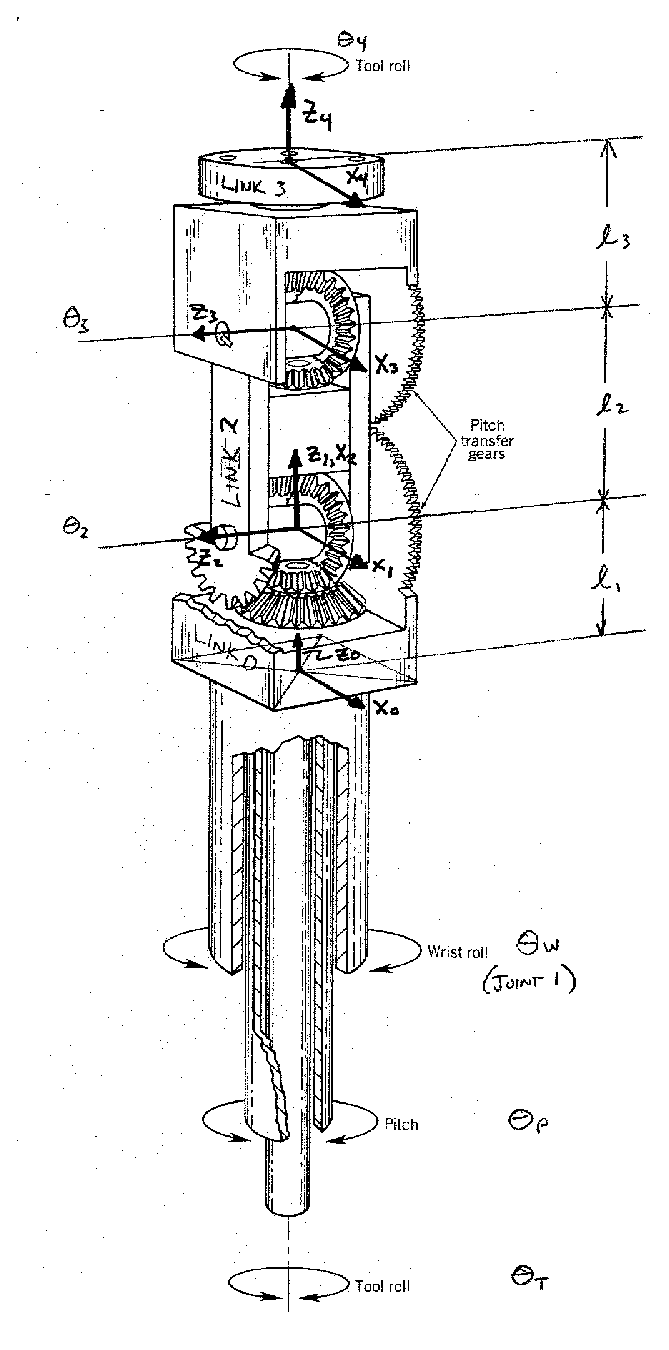
\includegraphics[width=5.38cm]{figs03/00423.eps}
\vspace{0.25in}

6) Following the procedures of Section \ref{DH_Steps}, we obtain
\vspace{0.25in}

\begin{tabular}{|c|c|c|c|c|} \hline
$N$	&  $\alpha_{N-1}$   &  $a_{N-1}$    	& $d_N$		&  $\theta_N$  \\     \hline
1	&   0 		    &    0 	    	&  $l_1$	&    $\theta_W$        \\ \hline
2	&   $\pi/2 $	    &    0       	&   0		& $\pi/2 + \theta_p$        	\\ \hline
3	&   0		    &   $l_2$		&  0		& $-\pi/2 + \theta_p$		\\ \hline
4	&   $-\pi/2 $       &   0		&  $l_3$	& $\theta_4$       		\\ \hline
\end{tabular}

Note that joints 2 and 3 form a single degree of freedom driven by $\theta_p$ because they are coupled together by the pitch transfer gears.

\end{ExampleCont}


\section{Spaces}

We have seen that the forward kinematics analysis generates a 4x4 matrix which is a function of $N$ variables where $N$ is the number of joints.   As the joints move to different values, the 4x4 matrix specifies different positions and orientations in the task space corresponding to a frame on the last link usually known as the end effector.

Although this matrix maps points in the end effector coordinate system to the base coordinate system, it is sometimes useful to think of this matrix as a description of a mapping from a set of joint values to an end effector configuration.   For a manipulator with $N$ joints, the joint values form a point in a $N$ dimensional space we call the {\it Joint Space}.

The 4x4 matrix $^0_NT$ gives us a rotation matrix and X,Y,Z coordinates of the end effector.  This is termed a ``configuration" of the manipulator end effector.   We commonly derive three orientation parameters such as roll, pitch, yaw, angles from the upper 3x3 part of $^0_NT$ to give six numbers which characterize the end effector configuration:

\begin{equation}
\left [
   \begin{array}{c}
	    X \\ Y \\ Z \\ \mathrm{roll} \\ \mathrm{pitch} \\ \mathrm{yaw}
   \end{array}
\right ]
\end{equation}

The above six numbers define a point in {\it End Effector Space}. End Effector Space is sometimes called ``Task Space" since it is a natural space in which to represent tasks or ``Configuration Space" although this term has a slightly different meaning in the context of motion planning.

As a manipulator moves around, a point moves around in joint space representing the values of its joints, and another point moves around in end effector space representing the configuration of the end effector.  As we shall see in the next chapter, there may be more than one joint space point which corresponds to the same end effector point, but there is always exactly one point in end effector space for each point in joint space.

Another relevant space is {\it Actuator Space}.   In most serial robots the actuators are located directly on each joint and actuator motion is a linear function of or is equal to the joint motion.   However in certain designs, such as the Yakusawa Motoman L-3, actuators may drive the joints through linkages and therefore move somewhat differently than the joints of the serial chain.  For good discussion of this consult Chapter 3 of Craig.


\newpage
\section{A further look at  the DH notation}
(The following section may be skipped without loss in future chapters)

\subsection{Structure of the Link Transform}

We can obtain some insight into the computation of link transformations by grouping the terms as shown in Figure \ref{LinkTransformBlobs}.  The clusters in Figure \ref{LinkTransformBlobs} represent blocks of terms which depend on a specific DH parameters.  Often, with industrial manipulators,
\[
\alpha_{i-1} = \{ 0, \pm \frac{\pi}{2}, \pi \}
\]
because they are easier to design and manufacture that way.   For these cases, we can see that the final expression for the link transform is simplified by $\cos(\alpha_{i-1}) = \{0,\pm1\}$.

Finally, we can classify the DH parameters into ones describing the {\it structure} of the link ($\theta_i, d_i$) versus the {\it relationship} with the next link ($\alpha_{i-1}, a_{i-1}$).  Each of these two classes has one rotational and one translational parameter:

\begin{center}
\begin{tabular}{r|cc}
            & Translation & Rotation \\ \hline
Structure   &  $a_{i-1}$ & $\alpha_{i-1}$  \\
Relationship &  $d_i$      & $\theta_i $    \\

\end{tabular}
\end{center}


\begin{figure}
\includegraphics[width=100mm]{figs03/00712.eps}
\caption{Different term types in the DH Link Transform). Matrix elements have dependencies on link {\it relationship} ($\theta_i, d_i$) or link {\it structure} ($\alpha_{i-1}, a_{i-1}$).}\label{LinkTransformBlobs}
\end{figure}


\subsection{Craig's vs. Paul's Transforms}\label{CraigVsPaul}

The first textbook on robot manpiulation was ``Robot Manipulators, Mathematics, Mechanics, and Control," by Richard Paul of the University of Pennsylvania (MIT Pres, 1981).    This book was very influential in starting research and courses around the world on robotic manipulation.   However, Paul used a slightly different variation on the Denavit Hartenberg method which results in different description of links.    In looking at the robotic manipulation literature, a researcher will still encounter work done in Paul's notation.

Both Craig and Paul's systems use the same DH parameters.  The key difference is that Paul's system puts the origin of frame N at the end of the link (point $B_{N+1}$ as defined in this chapter). Thus, different DH parameters are used in Paul's link description (Figure \ref{PaulTransformBlobs}).


\begin{figure}\centering
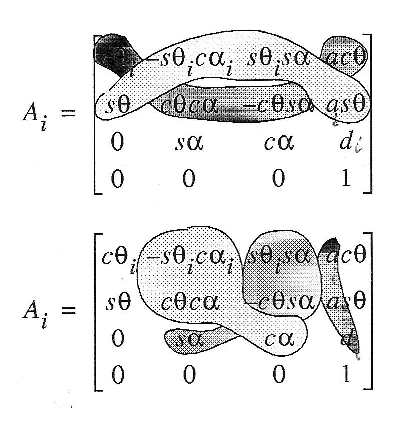
\includegraphics[width=60mm]{figs03/00713.eps}
\caption{Link transform for Paul's variation on the DH method.  Note different subscripts. Term types in the DH Link Transform similar to Figure \ref{LinkTransformBlobs}. }\label{PaulTransformBlobs}
\end{figure}


Paul's transform selects different DH parameters to represent the structure and relationships of the links:

\begin{center}
Paul's Link Parameters \\
\begin{tabular}{r|cc}
            & Translation & Rotation \\ \hline
Structure   &  $a_{i}$ & $\alpha_{i}$  \\
Relationship &  $d_i$      & $\theta_i $    \\
\end{tabular}
\end{center}

The obvious advantage of Paul's method is that subscripts are more consistent within the transform for each link.  However it has the non-intutive notion that the origin of Frame $N$ lies on axis $N+1$.  Craig's method has the more intuitive notion that  link frame $N$ is at the beginning of the link, located on axis $N$, but requires mixing of indeces in the link transform.  The two link frame assignment methods are summarized in Figure \ref{CraigPaulLinkFrames}.

\begin{figure}
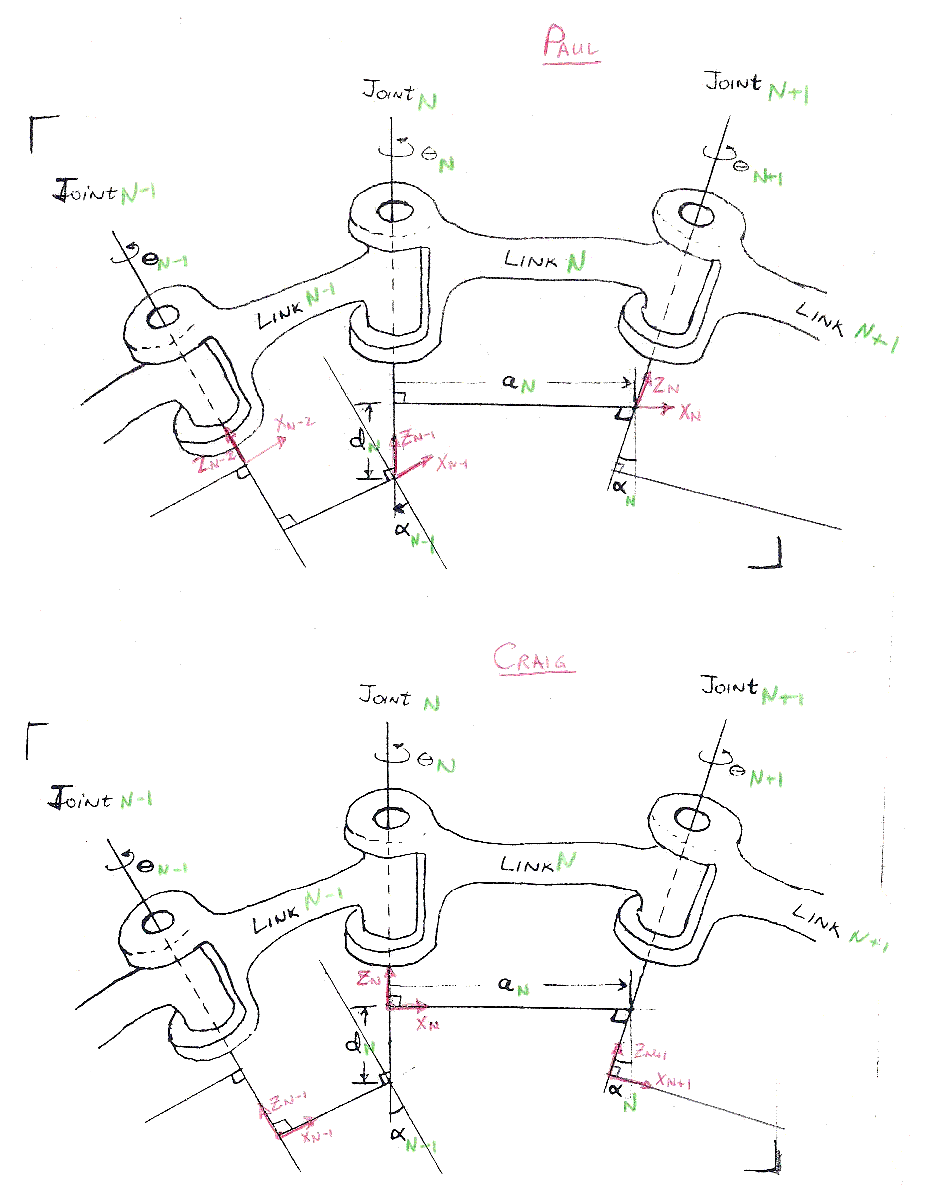
\includegraphics[width=150mm]{figs03/00714.eps}
\caption{Different link frame assignments (within the same DH parameters) for Craig (bottom) and Paul's (top)  methods.}\label{CraigPaulLinkFrames}
\end{figure}



%
% \section{Summary of Notation}
%
% \input{includes/notation03.tex}
